\chapter{Planung}
\section{Rollenverteilung}
\section{Anforderungen}
\section{Meilensteine}
\section{Architektur}
Bei dem ersten Treffen mit dem 'Kunden' wurde von uns eine Software zur Überwachung eines Raumes mithilfe einer herkömmlichen IP-Kamera gewünscht.
Da hierfür auch eine Möglichkeit zur Interaktion mit dem System gegeben sein sollte, entschieden wir uns für eine Webseite, mit welcher
der Videofeed sichtbar und Einstellungen vorgenommen werden sollten. Da die Software im Gegensatz zu anderen kommerziellen Produkten im lokalen Netz bleiben sollte,
spielte die Sicherheit keine große Rolle.\\
Die Architektur sollte die Aufteilung der Schichten wie Logik, Datenhaltung sowie die Präsentation durch den Webserver darstellen.
Hierfür wurde zuerst Abbildung \ref{img:architecture-sketch} erstellt.\\\\
\begin{figure}[h]
	\centering
	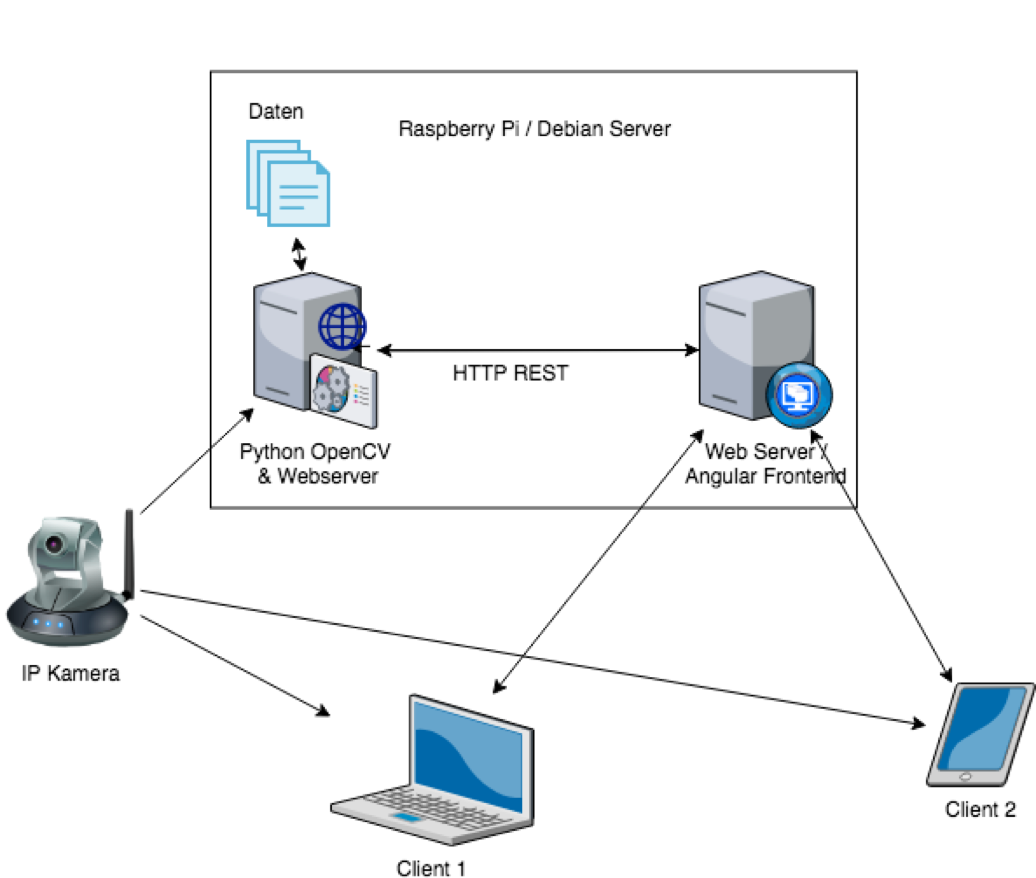
\includegraphics[height=10cm]{content/pictures/architecture-sketch.png}
	\caption{Erste Planung der Architektur}
	\label{img:architecture-sketch}
\end{figure}
Da der Architekt im Gebiet der Webtechnologien kaum Erfahrung hatte, entschieden die verantwortlichen Entwickler sich selbst für Angular und sprachen sich bei
der Entwicklung ab. Lediglich REST wurde für die Kommunikation zwischen Frontend und Backend definiert. 
Um die Aufteilung der Klassen und Kommunikation innerhalb des Backends darzustellen wurde ein grobes Klassendiagramm erstellt (Abbildung \ref{img:backend-classdiagramm}).\\\\
\begin{figure}[]
	\centering
	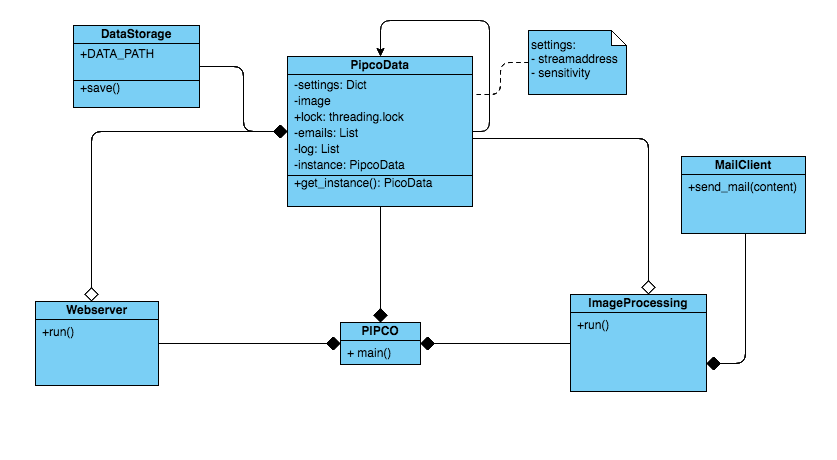
\includegraphics[width=\textwidth]{content/pictures/classdiagramm.png}
	\caption{Klassendiagramm Aufbau des Backends}
	\label{img:backend-classdiagramm}
\end{figure}
Für die Unabhängige Entwicklung der Kommunikation von Frontend und Backend wurde eine Liste mit den notwendigen REST-Nachrichten erstellt (Tabelle \ref{table:kommunikation}).\\\\
\begin{table}[]
	\centering
	\caption{Kommunikation Backend und Frontend}
	\label{table:kommunikation}
	\resizebox{\textwidth}{!}{\begin{tabular}{llll}
		\textbf{Type} & \textbf{address}                                                             & \textbf{keys}                                                                                                                                                                                                                                          & \textbf{returns}           \\
		POST          & /login                                                                       & user, password                                                                                                                                                                                                                                         & OK / Error 403             \\
		GET           & /videostream                                                                 &                                                                                                                                                                                                                                                        & mjpeg stream               \\
		GET           & /logs/\textless{}page\_no\textgreater{}/\textless{}batch\_size\textgreater{} &                                                                                                                                                                                                                                                        & list with logs             \\
		DELETE        & /log/\textless{}log\_id\textgreater{}                                        &                                                                                                                                                                                                                                                        & id / Error 403             \\
		POST          & /mail                                                                        &                                                                                                                                                                                                                                                        & id / Error 403             \\
		GET           & /mails                                                                       &                                                                                                                                                                                                                                                        & list of mail addresses     \\
		DELETE        & /mail/\textless{}mail\_id\textgreater{}                                      &                                                                                                                                                                                                                                                        & id / Error 403             \\
		PUT           & /mail/\textless{}mail\_id\textgreater{}                                      &                                                                                                                                                                                                                                                        & notify status / Error 403  \\
		POST          & /config                                                                      & \multirow{4}{*}{\begin{tabular}[c]{@{}l@{}}sensitivity(float), streamaddress,brightness (float),\\ contrast (float), log\_enabled(bool),\\ global\_notify(bool), cliplength (int in seconds),\\ max\_logs (int),max\_storage (int in MB)\end{tabular}} & changed values / Error 403 \\
		&                                                                              &                                                                                                                                                                                                                                                        &                            \\
		&                                                                              &                                                                                                                                                                                                                                                        &                            \\
		&                                                                              &                                                                                                                                                                                                                                                        &                            \\
		GET           & config                                                                       &                                                                                                                                                                                                                                                        & config                     \\
		GET           & /recording/\textless{}filename\textgreater{}                                 &                                                                                                                                                                                                                                                        & videofile                  \\
		GET           & /backup                                                                      &                                                                                                                                                                                                                                                        & backup.zip                 \\
		&                                                                              &                                                                                                                                                                                                                                                        &                           
	\end{tabular}}
\end{table}
Während der Entwicklung stellte sich heraus, dass der Aufwand für die Implementierung der bidirektionalen Kommunikation zwischen Frontend und Backend zu hoch ist, weshalb wir uns dazu entschieden die Daten direkt vom Backend zu holen und die Logs mithilfe von Polling aktuell zu halten.
Eine weitere Änderung war die Kamera, welche lediglich vom Backend angefragt wird. Der Client sollte sich ausschließlich die Bilder, mit eingezeichneten Bewegungen holen.
Hierdurch änderte sich die Architektur wie in Abbildung \ref{img:architecture-change} zu sehen.\\

Um den Ablauf besser nachvollziehen zu können wurde desweiteren ein Sequenzdiagramm erstellt (Abbildung \ref{img:sequencediagram}).

\begin{figure}[]
	\centering
	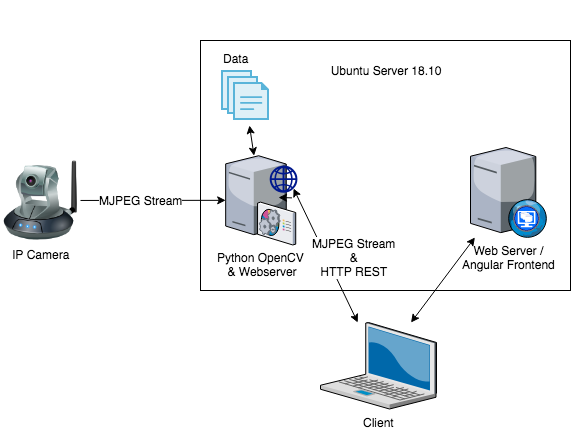
\includegraphics[width=\textwidth]{content/pictures/architecture-change.png}
	\caption{Klassendiagramm: Direkter Zugriff auf das Backend}
	\label{img:architecture-change}
\end{figure}

\begin{figure}[]
	\centering
	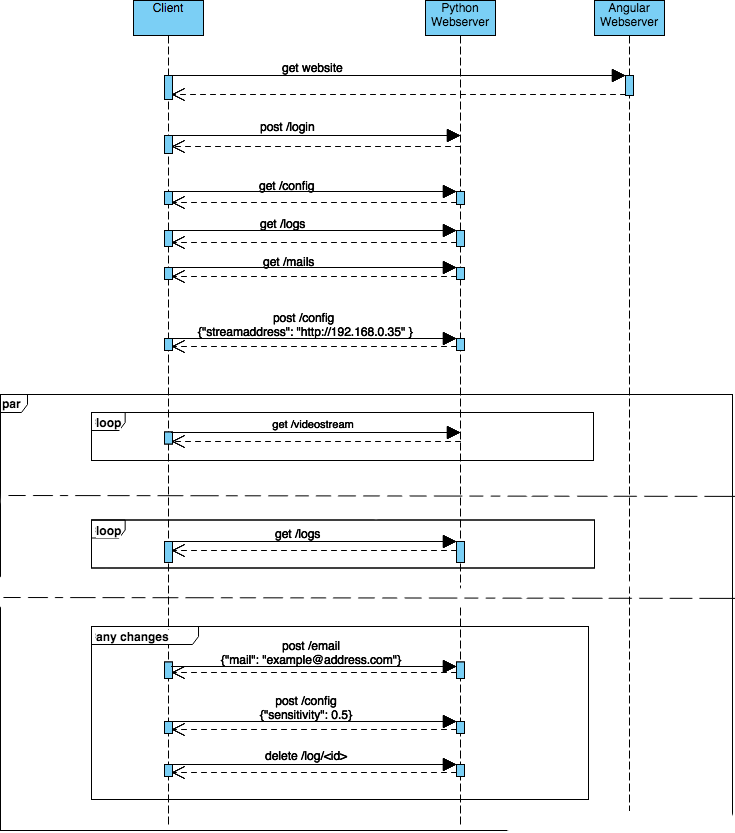
\includegraphics[width=\textwidth]{content/pictures/sequencediagram.png}
	\caption{Ablauf Login und Änderungen}
	\label{img:sequencediagram}
\end{figure}